\subsection{Das Optimierungsproblem}
Wie bereits erwähnt, ist durch die extrem hohe Anzahl an Parametern ein Durchprobieren aller Parameterkombinationen nicht möglich.
Es könnte kein Resultat in nützlicher Frist gefunden werden können.
Aus diesem Grund werden andere Verfahren verwendet, um das neuronale Netzwerk zu optimieren.
Alle diese Verfahren basieren auf dem Gradientenabstieg und werden in der Literatur oft auch 'Optimizer' genannt. Näheres zum Gradientenabstieg kann in Kapitel \textbf{xyz} gefunden werden.

Ein einfacher Algorithmus ist der stochastische Gradientenabstieg.
Der Abstiegsschritt 
\begin{equation}
p_{\text{new}}:=p-\eta \nabla \Lb_{i}(p)
\end{equation}
findet Parameterwerte $p_{\text{new}}$, für die der Fehler kleiner ist. Die Parameter $p$ stehen für sämtliche inneren Gewichte $w$ und Offsetwerte $b$. Die Schrittweite $\eta$ muss experimentell ermittelt und wird oft auch als \textit{learning rate} bezeichnet. Die Kunst liegt darin, $\eta$ so zu wählen, dass lokale Minima und Rauschen die Konvergenz nicht behindern. Der Algorithmus bricht erst ab, wenn ein Minimum erreicht ist oder die vorgegebene maximale Anzahl an Iterationen ausgeschöpft ist.
Die Fehlerfunktion
\begin{equation}
\Lb(w_1, \cdots, w_n, b_1, \cdots, b_n) = \Lb(p)=\sum_{i=1}^{n}\Lb_{i}(p)=\sum_{i=1}^{n}\Lb(\hat{y_i}-y_i)^2
\end{equation}
\begin{figure}
	\begin{center}
		\tikzstyle{inputNode}=[draw,circle,minimum size=17pt,inner sep=0pt]
\tikzstyle{stateTransition}=[-stealth, thick]

%\begin{document}
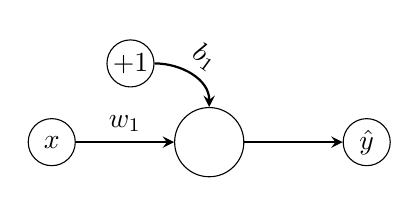
\begin{tikzpicture}
	\node[draw,circle,minimum size=25pt,inner sep=0pt] (x) at (0,0) {};

	\node[inputNode] (x0) at (-1, 1) {$\tiny +1$};
	\node[inputNode] (x1) at (-2, 0) {$\tiny x$};
	\node[inputNode] (y) at (2, 0) {$\tiny \hat{y}$};
	
	\draw[stateTransition] (x0) to[out=0,in=90] node [midway, sloped, above] {$b_{1}$} (x);
	\draw[stateTransition] (x1) to[out=0,in=180] node [midway, sloped, above] {$w_{1}$} (x);
	\draw[stateTransition] (x) to[out=0,in=180] node [midway, sloped, above] {} (y);

	
\end{tikzpicture}
		\caption{Übersicht eines Neuronalen Netzwerks}
		\label{ableitung:fig:single_neuron}
	\end{center}
\end{figure} 
berechnet den Fehler, welcher durch die $w$ und $b$ beeinflusst wird. Um die Konsequenzen der partiellen Ableitung nach den jeweiligen Parametern einzuführen, wird als Beispiel ein Netzwerk, entsprechend Abbildung \ref{ableitung:fig:single_neuron}, mit nur einem Neuron gewählt.
An diesem Beispiel
\begin{equation}
\hat{y} = \sigma \left( w_1 \cdot x + b_1 \right)
\end{equation}
lassen sich alle Effekte gut zeigen.
Dieses Netzwerk kann in die Fehlerfunktion $\Lb$, gemäss der Gleichung \ref{ableitung:eqn:loss_net}, eingesetzt werden. Die anschliessende Differentiation nach den inneren Parametern $w$ und $b$ führt zum Gradienten der beiden Parametern. Die neuen Parameter 
\begin{equation}
\begin{split}
\begin{bmatrix}w_{1}\\b_{1}\end{bmatrix}_{\text{new}}:&={\begin{bmatrix}w_{1}\\b_{1}\end{bmatrix}}-\eta {\begin{bmatrix}
{\frac {\partial }{\partial w_{1}}}(\sigma(w_{1}x_{i}+b_{1})-y_{i})^{2}\\
{\frac {\partial }{\partial b_{1}}}(\sigma(w_{1}x_{i}+b_{1})-y_{i})^{2}\end{bmatrix}} \\ & =
{\begin{bmatrix}w_{1}\\b_{1}\end{bmatrix}}-\eta {\begin{bmatrix}2(\sigma(w_{1}x_{i}+b_{1}) - y_i) \cdot \sigma'(w_{1}x_{i}+b_{1}) \cdot (w_{1}x_{i}+b_{1}) x_{i} \\2(\sigma(w_{1}x_{i}+b_{1}) - y_i) \cdot \sigma'(w_{1}x_{i}+b_{1}) \cdot (w_{1}x_{i}+b_{1}) \end{bmatrix}}
\end{split}
\end{equation}
werden nach vollziehen des Gradientenabstiegs in jeder Iteration aktualisiert.
Dieses Beispiel mit einem Neuron zeigt auf, dass, dass mit steigender Netzkomplexität die Terme noch viel grösser werden. Dies ist auf die Kettenregel $u'(v(x)) = u'(v(x)) \cdot (v'(x))$ zurückzuführen. Mit diesem Verfahren ist der Gradientenabstieg zwar möglich, jedoch sehr rechenintensiv. Aus diesem Grunde verwenden die meisten Frameworks den Backpropagation-Algorithmus, welcher etwas effizienter ist.